\subsection{Scaled boundary finite element method in 2D elasticity}
\paragraph{}
The SBFEM is reviewed briefly in this section for two-dimensional elasticity.
Detailed derivation can be found in literature \cite{Wolf1996, WOLF20015551, Deeks2002}.
In the SBFEM, a scaling center O is selected at a point from which the whole boundary of the domain is visible (scaling requirement) (see Fig.~\ref{lr_fig:nurbs_rational_basis}).
The boundary of the domain can be represented with conventional finite elements as shown in Fig.~\ref{lr_fig:nurbs_rational_basis}.
The geometry of the domain has only to satisfy the scaling requirement.
This condition is automatically satisfied for all convex polygons and many concave polygons.
The scaling requirement is equivalent to the notion of `star convexity' \cite{Bishop2014}.
For the domain that does not meet the scaling requirement, the requirement can always be satisfied by sub-structuring, i.e. dividing the structure into smaller subdomains, for example, scaled boundary polygon formulation \cite{NATARAJAN2014101}.
\begin{figure}[!ht]
    \centering
    \scalebox{0.4}{
        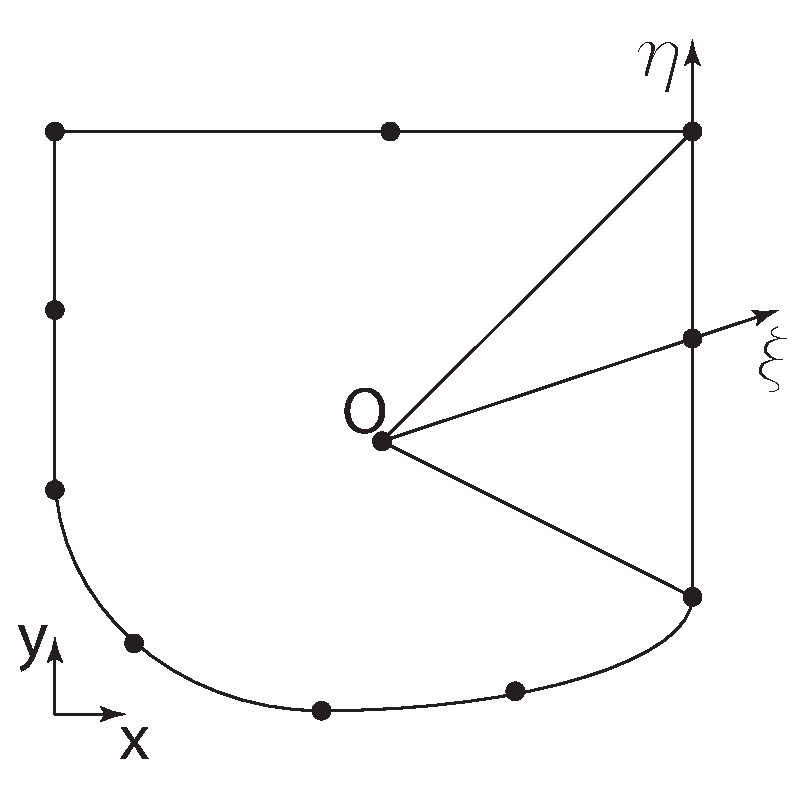
\includegraphics{literature/images/lr_sbfem_desc.eps}
    }
    \label{lr_fig:sbfem_desc}
    \caption{Two dimensional scaled boundary coordinates, where O is the scaling center and $\xi$ is the radial coordinate with $\xi=0$ at the scaling center and $\xi=1$ on the boundary.}
\end{figure}

The nodal coordinates on the boundary are denoted as $\mathbf{x}_b$. As in a standard 1D iso-parametric finite element, the geometry of the element described by the coordinates $\mathbf{x}_b(η)$, is expressed as
\begin{equation}
    \mathbf{x}_b(\eta) = \mathbf{N}(\eta) \mathbf{x}_b
    \label{lr_eq:sbfem_boundary_interpolate}
\end{equation}

where $\mathbf{N}(\eta)$ is the shape function matrix.
Without loss of generality, the origin of the Cartesian coordinate system is chosen at the scaling center.
The geometry of the subdomain, described by $x$, is formed by scaling the boundary (Eq.~\ref{lr_eq:sbfem_boundary_interpolate})
\begin{equation}
    \mathbf{x} = \xi \mathbf{x}_b (\eta)
\end{equation}

where $\xi$ is the normalized radial coordinate running from the scaling center towards the boundary, with $\xi=0$ at the scaling center and $\xi=1$ on the boundary.
The coordinates $\xi$ and $\eta$ are the so-called scaled boundary coordinates.
They are related to the polar coordinates $r$ and $\theta$.
The transformation is expressed as
\begin{equation}
\begin{aligned}
    r(\xi,\eta) &= \xi r_b(\eta)     \\
    \theta(\eta) &= \arctan \frac{y(\eta)}{x(\eta)}
\end{aligned}
\end{equation}

where $r_b$ is the distance from the scaling center to a point on the boundary.
The transformation between the Cartesian coordinates and the scaled boundary coordinates is similar to the coordinate transformation in the constructing iso-parametric finite elements.

The displacement at any point are approximated by
\begin{equation}
    \mathbf{u}(\xi,\eta) = \mathbf{N}(\eta) \mathbf{u}(\xi)
    \label{lr_eq:sbfem_disp_interpolation}
\end{equation}

where $\mathbf{N}(\eta)$ are the shape functions of elements on the boundary and $\mathbf{u(\xi)}$ is the displacement along the radial lines, represented by a set of N analytical functions.
By substituting Eq.~\ref{lr_eq:sbfem_disp_interpolation} into the definition of strain-displacement relations, the strain $\epsilon(\xi,\eta)$ are expressed as
\begin{equation}
    \epsilon(\xi,\eta) = \mathbf{Lu}(\xi,\eta)
    \label{lr_eq:sbfem_strain_disp_relation}
\end{equation}

where $\mathbf{L}$ is a linear operator matrix formulated in the scaled boundary coordinates
\begin{equation}
    \mathbf{L} =    \mathbf{b}_1(\eta) \frac{\partial}{\partial \xi} +
                    \frac{1}{\xi} \mathbf{b}_2(\eta)
    \label{lr_eq:sbfem_l_operator}
\end{equation}

and
\begin{equation}
    \begin{aligned}
    \mathbf{b}_1(\eta) & = \frac{1}{|J|}
            \begin{bmatrix}
                y_b(\eta),_{\eta}   &   0   \\
                0   &   -x_b(\eta),_{\eta}  \\
                -x_b(\eta),_{\eta} & y_b(\eta),_{\eta}
            \end{bmatrix} \\
    \mathbf{b}_2(\eta) & = \frac{1}{|J|}
            \begin{bmatrix}
                -y_b    &   0   \\
                0       &   x_b \\
                x_b     &   y_b
            \end{bmatrix}
    \end{aligned}
    \label{lr_eq:sbfem_little_b}
\end{equation}

The determinant of the Jacobian matrix is
\begin{equation}
    |J| = x_b(\eta)y_b(\eta),_{\eta}
        - y_b(\eta)x_b(\eta),_{\eta}
    \label{lr_eq:sbfem_Jdet}
\end{equation}

where $x_b(\eta)$ and $y_b(\eta)$ are given by Eq.~\ref{lr_eq:sbfem_boundary_interpolate}.
The stresses $\sigma(\xi,\eta)$ are given by:
\begin{equation}
    \sigma(\xi,\eta) =  \mathbf{DB}_1(\eta) \mathbf{u}(\xi),_{\xi} +
                        \frac{1}{\xi} \mathbf{DB}_2(\eta) \mathbf{u}(\xi)
    \label{lr_eq:sbfem_stress}
\end{equation}

where in the above equation, the definition of strain and the linear operator matrix given by Eq.~\ref{lr_eq:sbfem_strain_disp_relation} and Eq.~\ref{lr_eq:sbfem_l_operator} are used with
\begin{equation}
    \begin{aligned}
        \mathbf{B}_1(\eta) &= \mathbf{b}_1(\eta) \mathbf{N}(\eta)    \\
        \mathbf{B}_2(\eta) &= \mathbf{b}_2(\eta) \mathbf{N}(\eta),_{\eta}
        \label{lr_eq:sbfem_captial_b}
    \end{aligned}
\end{equation}

substituting Eq.~\ref{lr_eq:sbfem_strain_disp_relation} and Eq.~\ref{lr_eq:sbfem_stress} in the virtual work statement for elastostatics and following the derivation in \cite{Deeks2002}
\begin{equation}
    \begin{aligned}
        \delta \mathbf{u}(\xi)^{T} \left(
            (\mathbf{E}_0 \xi \mathbf{u}(\xi),_{\xi}
            + \mathbf{E}_1^T \mathbf{u}(\xi))|_{\xi=1}
            - \mathbf{F}
        \right) - \\
        \int_0^1 \delta u(\xi)^T\left(
            \mathbf{E}_0 \xi^2 \mathbf{u}(\xi),_{\xi\xi} + (\mathbf{E}_0 + \mathbf{E}_1^T - \mathbf{E}_1) \xi \mathbf{u}(\xi),_{\xi}
            - \mathbf{E}_2 u(\xi)
        \right) d\xi = 0
    \end{aligned}
    \label{lr_eq:sbfem_virtual_work}
\end{equation}

where $\mathbf{u}(\xi)$ is the nodal displacement vector and $\mathbf{F}$ is the vector of equivalent boundary nodal forces, given by:
\begin{equation}
    \mathbf{F} = (\mathbf{E}_0 \xi \mathbf{u}(\xi),_{\xi} + \mathbf{E}_1^T \mathbf{u}(\xi))|_{\xi=1}
    \label{lr_eq:sbfem_nodal forces}
\end{equation}

By considering the arbitrariness of $\delta \mathbf{u}(\xi)$, the following ODE is obtained:
\begin{equation}
    \mathbf{E}_0 \xi^2 \mathbf{u}(\xi),{\xi\xi} + (\mathbf{E}_0 + \mathbf{E}_1^T - \mathbf{E}_1)\xi \mathbf{u}(\xi),_{\xi} - \mathbf{E}_2 \mathbf{u}(\xi) = 0
    \label{lr_eq:sbfem_ODE}
\end{equation}

where $\mathbf{E}_0$, $\mathbf{E}_1$ and $\mathbf{E}_2$ are known as the coefficient matrices and are given by:
\begin{equation}
    \begin{aligned}
        \mathbf{E}_0 &= \int_\eta \mathbf{B}_1(\eta)^T \mathbf{DB}_1(\eta)|J|d\eta \\
        \mathbf{E}_1 &= \int_\eta \mathbf{B}_2(\eta)^T \mathbf{DB}_1(\eta)|J|d\eta \\
        \mathbf{E}_2 &= \int_\eta \mathbf{B}_2(\eta)^T \mathbf{DB}_2(\eta)|J|d\eta
    \end{aligned}
    \label{lr_eq:sbfem_coe_matrix}
\end{equation}

Eq.~\ref{lr_eq:sbfem_ODE} is a homogeneous second-order differential equation.
Its solution is obtained by introducing the variable $\mathbf{\chi}(\xi)$
\begin{equation}
    \mathbf{\chi} = \left\{
        \begin{matrix}
            \mathbf{u}(\xi)  \\
            \mathbf{q}(\xi)
        \end{matrix}
    \right\}
    \label{lr_eq:sbfem_ODE_soltion}
\end{equation}

where $\mathbf{q}(\xi)$ is the internal force vector
\begin{equation}
    \mathbf{q}(\xi) =   \mathbf{E}_0 \xi \mathbf{u}(\xi),_{\xi} +
                        \mathbf{E}_1^T \mathbf{u}(\xi)
    \label{lr_eq:sbfem_internal_force}
\end{equation}

The boundary nodal forces are related to the displacement functions by:
\begin{equation}
    \mathbf{F} = \mathbf{q}(\xi=1) = (\mathbf{E}_0\xi \mathbf{u}(\xi),_{\xi} + \mathbf{E}_1^T\mathbf{u}(\xi))|_{\xi=1}
    \label{lr_eq:sbfem_boundary_nodal_force}
\end{equation}

This allows Eq.~\ref{lr_eq:sbfem_ODE} to be transformed into a first order ordinary differential equation with twice the number of unknowns as:
\begin{equation}
    \xi \mathbf{\chi}(\xi),_{\xi} = -\mathbf{Z} \mathbf{\chi}(\xi)
    \label{lr_eq:sbfem_1stODE}
\end{equation}

where $\mathbf{Z}$ is a Hamiltonian matrix
\begin{equation}
    \mathbf{Z} = \begin{bmatrix}
        \mathbf{E}_0^{-1} \mathbf{E}_1^T    &  -\mathbf{E}_0^{-1}   \\
        \mathbf{E}_1 \mathbf{E}_0^{-1} \mathbf{E}_1^T - \mathbf{E}_2    &   -\mathbf{E}_1 \mathbf{E}_0^{-1}
    \end{bmatrix}
    \label{lr_eq:sbfem_zmatrix}
\end{equation}

An eigenvalue decomposition of $\mathbf{Z}$ is performed and it yields:
\begin{equation}
    \mathbf{Z} \begin{bmatrix}
        \mathbf{\Phi}_u \\
        \mathbf{\Phi}_q
    \end{bmatrix} = \begin{bmatrix}
        \mathbf{\Phi}_u  \\
        \mathbf{\Phi}_q
    \end{bmatrix} \mathbf{\Lambda}_n
    \label{lr_eq:sbfem_eigen_decomp}
\end{equation}

In Eq.~\ref{lr_eq:sbfem_eigen_decomp}, $\mathbf{\Lambda}_n$ $=$ diag$(\lambda_1$, $\lambda_2$, $\dots$, $\lambda_n)$ contains only the eigenvalues with negative real part.
$\mathbf{\Phi}_u$ and $\mathbf{\Phi}_q$ are the subsets of the eigenvectors corresponding to $\mathbf{Lambda}_n$.
They represent the modal displacements and forces, respectively.
The general solution of Eq.~\ref{lr_eq:sbfem_1stODE} is given by:
\begin{align}
    \mathbf{u}(\xi) &= \mathbf{\Phi}_u \xi^{-\mathbf{\Lambda_n}} \mathbf{c}
    \label{lr_eq:sbfem_general_sol_disp} \\
    \mathbf{q}(\xi) &= \mathbf{\Phi}_q \xi^{-\mathbf{\Lambda_n}} \mathbf{c}
    \label{lr_eq:sbfem_general_sol_str}
\end{align}

where $\mathbf{c}$ are integration constants that are obtained from the nodal displacements $\mathbf{u}_b = \mathbf{u}(\xi=1)$ as:
\begin{equation}
    \mathbf{c} = \mathbf{\Phi}_u^{-1} \mathbf{u}_b
    \label{lr_eq:sbfem_int_constant}
\end{equation}

The complete displacement field of a point defined by the sector covered by a line element on the boundary is obtained by substituting Eq.~\ref{lr_eq:sbfem_general_sol_str} into Eq.~\ref{lr_eq:sbfem_disp_interpolation} resulting in:
\begin{equation}
    \mathbf{u}(\xi,\eta) = \mathbf{R}(\eta) \mathbf{\Phi}_u \xi ^{-\mathbf{\Lambda}_n} c
    \label{lr_eq:sbfem_displacement_field}
\end{equation}

Taking the derivative of $\mathbf{u}(\xi)$ with respect to $\xi$ and substituting into Eq.~\ref{lr_eq:sbfem_stress} the stress field $\sigma(\xi,\eta)$ can be expressed as:
\begin{equation}
    \mathbf{\sigma}(\xi,\eta) = \mathbf{\Psi}_\alpha (\eta) \xi^{-\mathbf\Lambda}_n - \mathbf{I} \mathbf{c}
    \label{lr_eq:sbfem_stress_field}
\end{equation}

where the stress mode $\mathbf{\Psi}_\sigma(\eta)$ is defined as:
\begin{equation}
    \mathbf{\Psi}_\alpha(\eta) =    \mathbf{D}(
                                       -\mathbf{B}_1(\eta) \mathbf{\Phi}_u \mathbf{\Lambda}_n +
                                        \mathbf{B}_2(\eta) \mathbf{\Phi}_u
                                    )
    \label{lr_eq:sbfem_stress_mode}
\end{equation}

The stiffness matrix of an element is obtained by first substituting Eq.~\ref{lr_eq:sbfem_int_constant} into Eq.~\ref{lr_eq:sbfem_general_sol_str} at $\xi=1$.
This results in:
\begin{equation}
    \mathbf{F} = \mathbf{\Phi}_q \mathbf{\Phi}_u^{-1} \mathbf{u}_b
    \label{lr_eq:sbfem_kmat_previous}
\end{equation}

From Eq.~\ref{lr_eq:sbfem_kmat_previous}, the stiffness matrix $\mathbf{K}$ can be identified to be given by the expression
\begin{equation}
    \mathbf{K} = \mathbf{\Phi}_q \mathbf{\Phi}_u^{-1}
    \label{lr_eq:sbfem_kmat}
\end{equation}

The SBFEM has recently been extended to dynamic analysis in bounded domains \cite{Song2009}.
Assuming time-harmonic behavior, the scaled boundary equation in displacement is extended as:
\begin{equation}
    \mathbf{E}_0 \xi^2 \mathbf{u}(\xi),_{\xi\xi} +
    (\mathbf{E}_0 + \mathbf{E}_1^T - \mathbf{E}_1)\xi \mathbf{u}(\xi),_{\xi} -
    \mathbf{E}_2 \mathbf{u}(\xi) + \omega^2 \mathbf{M}_0 \xi^2 \mathbf{u}(\xi) = 0
    \label{lr_eq:sbfem_dynamic}
\end{equation}

Where $\mathbf{M}_0$ is a coefficient matrix defined as
\begin{equation}
    \mathbf{M}_0 = \int_\eta \mathbf{N}^T \rho \mathbf{N}|J| d\eta
    \label{lr_eq:sbfem_dynamic_mass}
\end{equation}

Using Eq.~\ref{lr_eq:sbfem_internal_force} and Eq.~\ref{lr_eq:sbfem_boundary_nodal_force}, Eq.~\ref{lr_eq:sbfem_dynamic_mass} can be transformed into an equivalent first-order non-linear differential equation in dynamic stiffness $\mathbf{S}(\omega)$,
\begin{equation}
    (\mathbf{S}(\omega)-\mathbf{E}_1)\mathbf{E}_0^{-1}
    (\mathbf{S}(\omega)-\mathbf{E}_1^T) - \mathbf{E}_2 +
    \omega \mathbf{S}(\omega),_\omega + \omega^2 \mathbf{M}_0 = 0
    \label{lr_eq:sbfem_dynamic_1stODE}
\end{equation}

The dynamic stiffness matrix $\mathbf{S}(\omega)$ relates the nodal forces to the displacements at the boundary as,
\begin{equation}
    \mathbf{F} = \mathbf{S}(\omega) \mathbf{u}(\xi=1)
    \label{lr_eq:sbfem_dynamic_nodal_force}
\end{equation}

Eq.~\ref{lr_eq:sbfem_dynamic_1stODE} is solved by expanding the dynamic stiffness into a series of continued fractions.
For this purpose, it is expressed as
\begin{equation}
    \mathbf{S}(\omega) = \mathbf{K} - \omega^2 \mathbf{M} + \omega^4 \left[
        \mathbf{R}^{(1)}    
    \right]^{-1}
    \label{lr_eq:sbfem_dynamic_stiffness}
\end{equation}

In Eq.~\ref{lr_eq:sbfem_dynamic_stiffness}, the first two terms represent the low-frequency expansion of the dynamic stiffness, whereas the third term corresponds to the residual of the low-frequency approximation.
Substituting Eq.~\ref{lr_eq:sbfem_dynamic_stiffness} in Eq.~\ref{lr_eq:sbfem_dynamic_1stODE} and equating terms in increasing order of powers of ω to zero yields equations for $\mathbf{K}$ ,$\mathbf{M}$  and $\mathbf{R}^{(1)}$.
Setting the constant terms equal to zero yields an algebraic Riccati equation for the static stiffness matrix $\mathbf{K}$, which is equivalent to the solution process described earlier.
Setting all terms in $\omega^2$ equal to zero yields a Lyapunov equation for the low-order mass matrix $\mathbf{M}$.
The solution procedure of that Lyapunov equation is described in detail in \cite{Son1997}.
The remaining equation for the residual is solved by expanding  $\mathbf{R}^{(1)}$ as
\begin{equation}
    \mathbf{R}^{(1)} = \mathbf{S}_0^{(1)} - \omega^2 \mathbf{S}_1^{(1)} + \omega^4 [\mathbf{R}^{(2)}]^{-1}
    \label{lr_eq:sbfem_dynamic_R}
\end{equation}

Eq.~\ref{lr_eq:sbfem_dynamic_R} is analogous to the expansion of the dynamic stiffness, Eq.~\ref{lr_eq:sbfem_dynamic_stiffness}, where the coefficients $\mathbf{S}^{(1)}_0$ and $\mathbf{S}^{(1)}_1$ correspond to the `stiffness' and `mass' term of $\mathbf{R}^{(1)}$, respectively.
Equations for $\mathbf{S}^{(1)}_0$ and $\mathbf{S}^{(1)}_1$ are found by substituting Eq.~\ref{lr_eq:sbfem_dynamic_R} into the equation for $\mathbf{R}^{(1)}$.
This procedure is continued until the residual $\mathbf{R}^{M_{cf}+1}$ can be neglected.
The symbol of $M_{cf}$ denotes the order of continued-fraction expansion.
Substituting all terms of the expansion back int Eq.~\ref{lr_eq:sbfem_dynamic_stiffness} yields:
\begin{dmath}
    \mathbf{S}(\omega) =    \mathbf{K} - \omega^2 \mathbf{M} + \omega^4 \left(
                                \mathbf{S}_0^{(1)} - \omega^2 \mathbf{S}^{(1)} + \omega^4 \left(
                                    \mathbf{S}_0^{(2)} - \omega^2 \mathbf{S}^{(2)} + \dots + 
                                    \omega^4 \left(
                                        \mathbf{S}_0^{(M_{cf})} - \omega^2 \mathbf{S}_1^{(M_{cf})}
                                    \right)^{-1}
                                \right)^{-1}
                            \right)^{-1}
\label{lr_eq:sbfem_dynamic_s_full}
\end{dmath}

The coefficients $\mathbf{S}^{(i)}_0$ and $\mathbf{S}^{(i)}_1$ in Eq.~\ref{lr_eq:sbfem_dynamic_s_full} are calculated following a recursive procedure.
A more detailed derivation can be found in \cite{Song2009}.